\section{New results}
\subsection{N16P16}

\begin{frame}
\tableofcontents[currentsection]
\end{frame}

\begin{frame}
\frametitle{Potenziale N16P16}
\begin{columns}

\begin{column}{0.3 \textwidth}
\begin{center}
\begin{figure}[!h]
         \subfigure[Coeff Si]
          {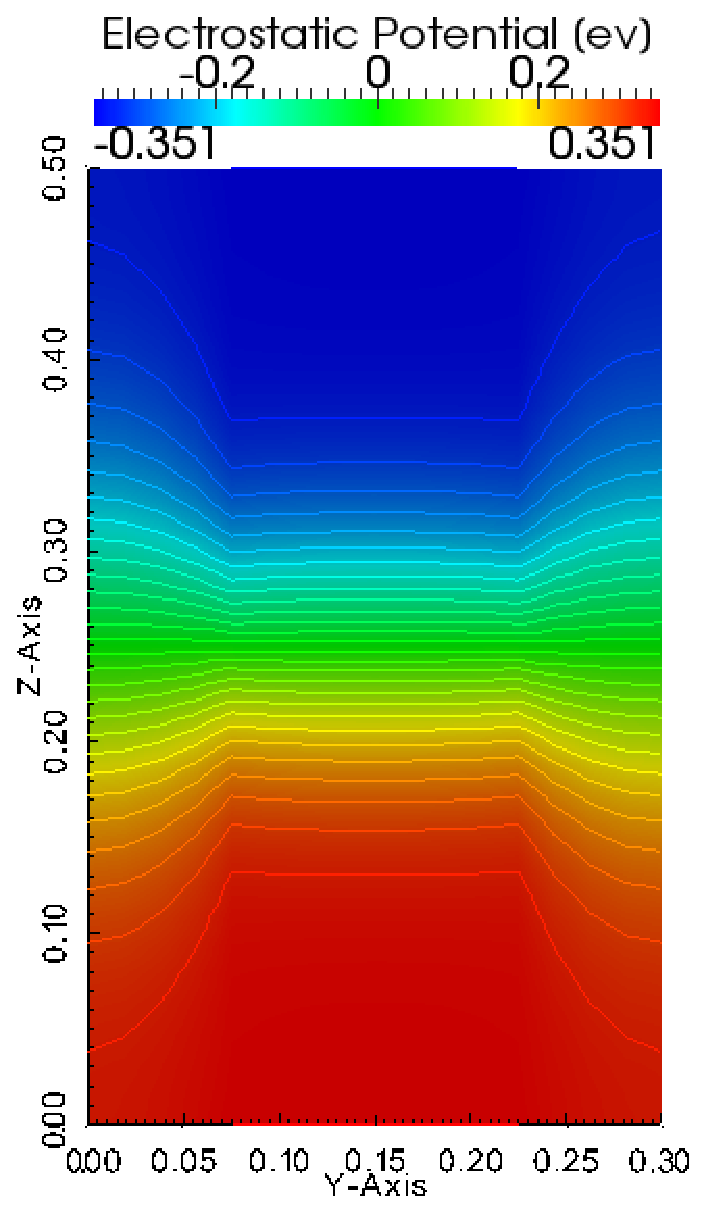
\includegraphics[scale=0.2]{N16P16YZ_coeffSi}}
          \end{figure}
\end{center}
\end{column}

\begin{column}{0.3 \textwidth}
\begin{center}
\begin{figure}[!h]
         \subfigure[Coeff Ox]
          {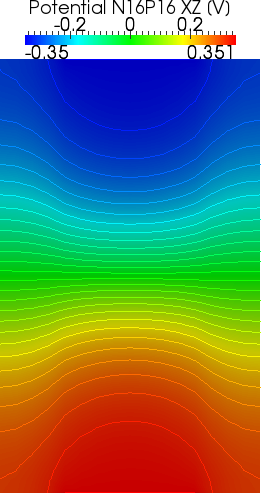
\includegraphics[scale=0.22]{N16P16XZ}}
\end{figure}
\end{center}
\end{column}

\begin{column}{0.3 \textwidth}
\begin{center}
\begin{figure}[!h]
         \subfigure[Sdevice]
          {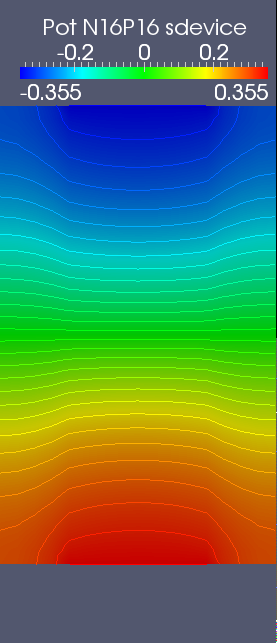
\includegraphics[scale=0.22]{N16P16sdeviceSLICE}}
\end{figure}
\end{center}
\end{column}

\end{columns}

\end{frame}

\begin{frame}
\frametitle{Potenziale tagli N16P16}

\begin{columns}

\begin{column}{0.25 \textwidth}
\begin{center}
\begin{figure}[!h]
         \subfigure[X=Y=0.15]
          {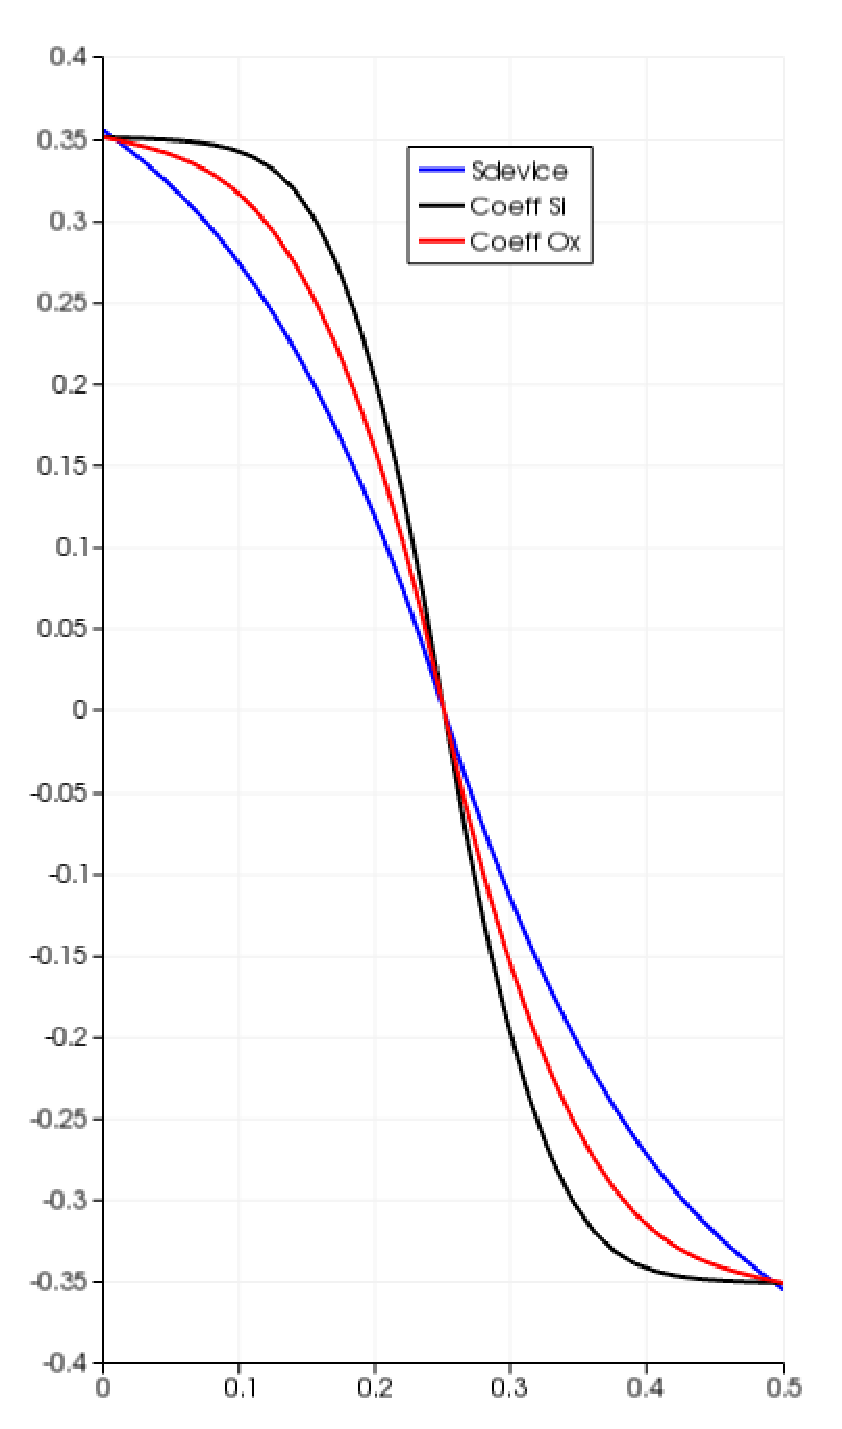
\includegraphics[scale=0.2]{N16P16_POT_Z}}
          \end{figure}
\end{center}
\end{column}

\begin{column}{0.25 \textwidth}
\begin{center}
\begin{figure}[!h]
         \subfigure[X=0.15 Z=0.2]
          {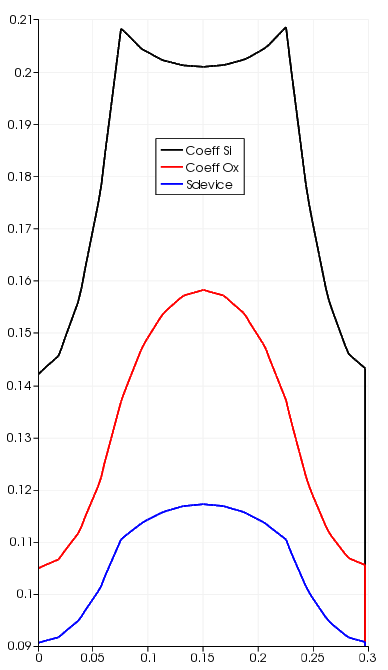
\includegraphics[scale=0.2]{N16P16_POT_Z02}}
\end{figure}
\end{center}
\end{column}

\begin{column}{0.25 \textwidth}
\begin{center}
\begin{figure}[!h]
         \subfigure[X=0.15 Z=0.25]
          {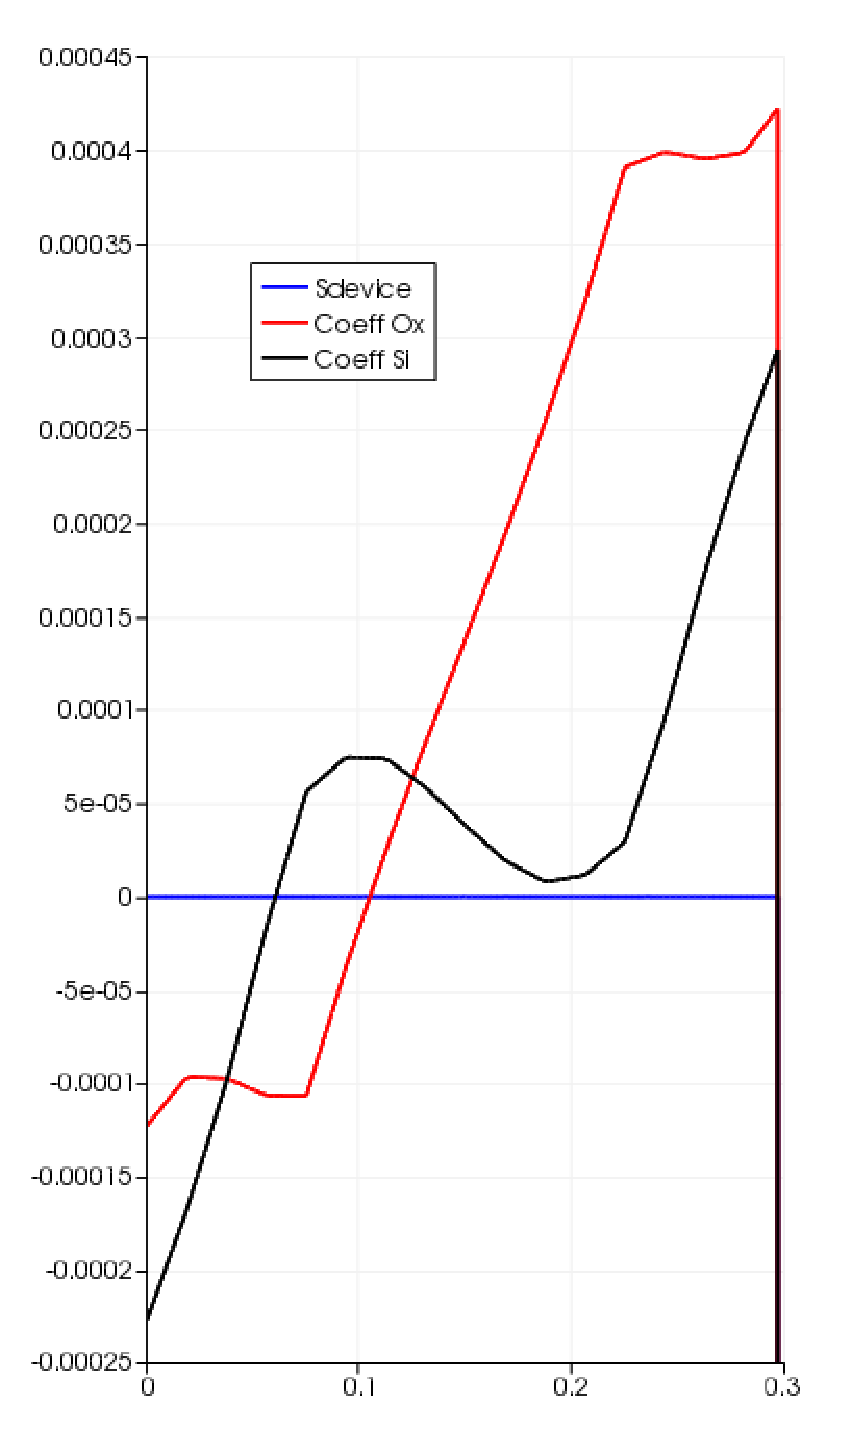
\includegraphics[scale=0.2]{N16P16_POT_Z025}}
\end{figure}
\end{center}
\end{column}

\begin{column}{0.25 \textwidth}
\begin{center}
\begin{figure}[!h]
         \subfigure[X=0.15 Z=0.48]
          {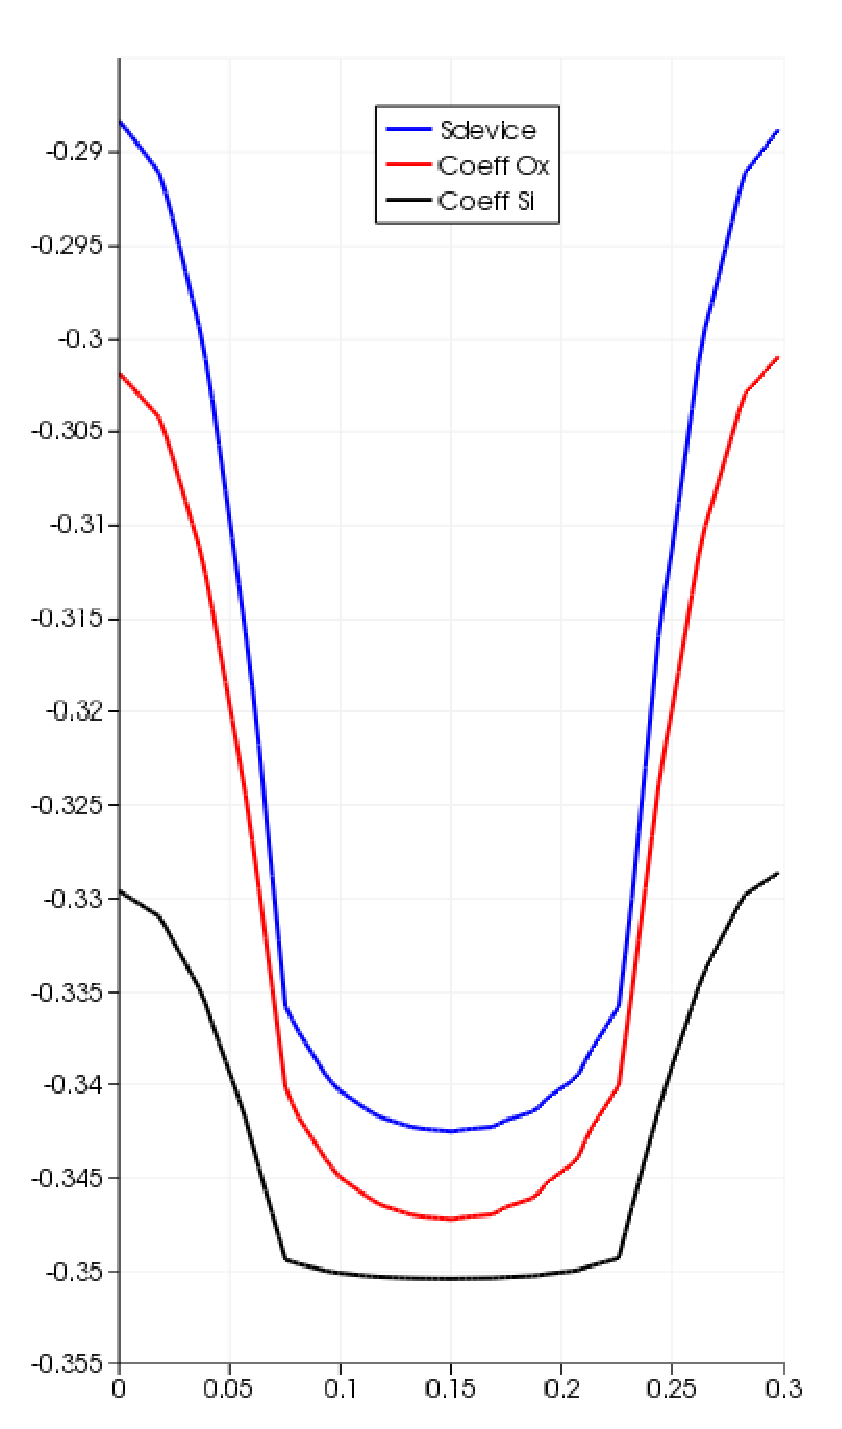
\includegraphics[scale=0.2]{N16P16_POT_Z048}}
\end{figure}
\end{center}
\end{column}

\end{columns}
\end{frame}



%----------------------------------------


\begin{frame}
\frametitle{Potenziale N16P16}
\begin{columns}

\begin{column}{0.3 \textwidth}
\begin{center}
\begin{figure}[!h]
          {\includegraphics[scale=0.25]{PNOX/N16P16/PotentialCoeffSI}}
          \end{figure}
\end{center}
\end{column}

\begin{column}{0.3 \textwidth}
\begin{center}
\begin{figure}[!h]
          {\includegraphics[scale=0.25]{PNOX/N16P16/PotentialCoeffOX}}
\end{figure}
\end{center}
\end{column}

\begin{column}{0.3 \textwidth}
\begin{center}
\begin{figure}[!h]
          {\includegraphics[scale=0.25]{PNOX/N16P16/PotentialSdevice}}
\end{figure}
\end{center}
\end{column}

\end{columns}

\end{frame}

\begin{frame}
\frametitle{Potenziale tagli N16P16}
\begin{columns}

\begin{column}{0.3 \textwidth}
\begin{center}
\begin{figure}[!h]
         \subfigure[X=Y=0.15]
          {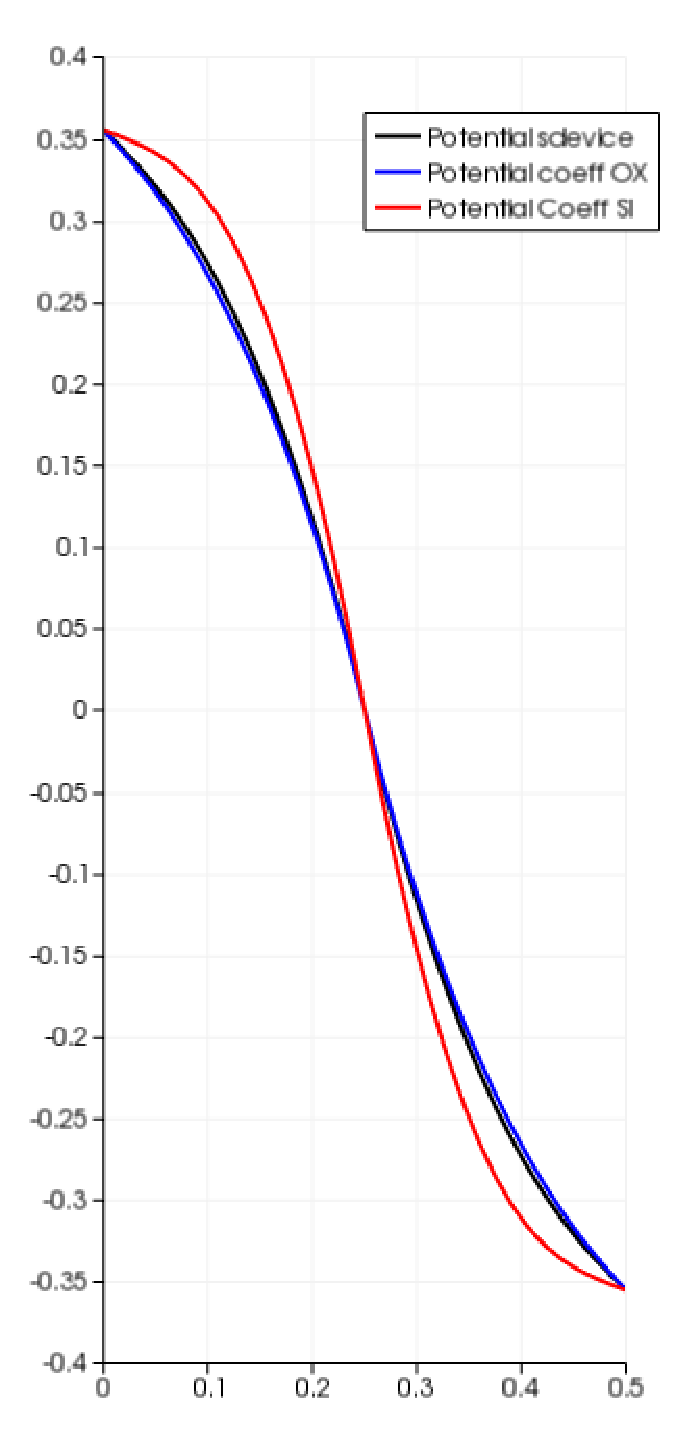
\includegraphics[scale=0.25]{PNOX/N16P16/Pot_Z}}
          \end{figure}
\end{center}
\end{column}

\begin{column}{0.3 \textwidth}
\begin{center}
\begin{figure}[!h]
         \subfigure[X=0.15 Z=0.25]
          {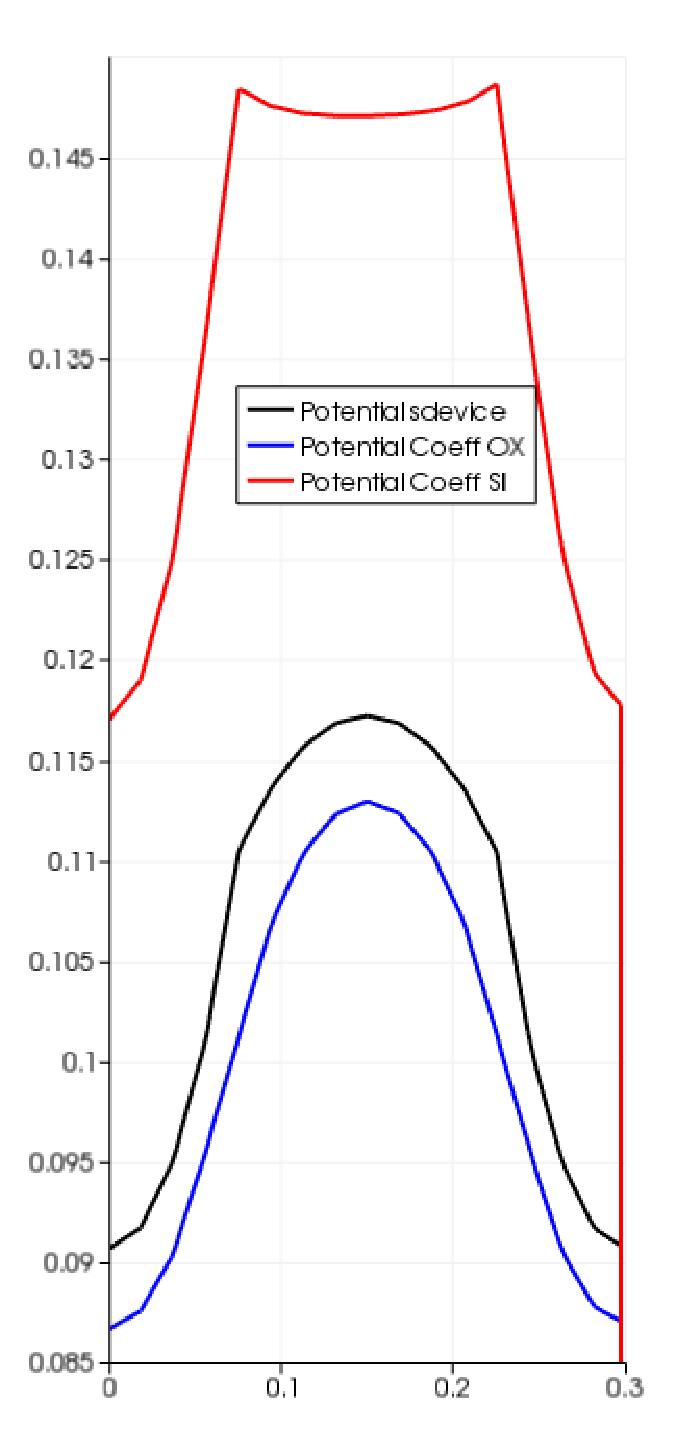
\includegraphics[scale=0.2]{PNOX/N16P16/Pot_Y_Z02}}
\end{figure}
\end{center}
\end{column}

\begin{column}{0.3 \textwidth}
\begin{center}
\begin{figure}[!h]
         \subfigure[X=0.15 Z=0.0]
          {\includegraphics[scale=0.25]{PNOX/N16P16/Pot_Y_Z00}}
\end{figure}
\end{center}
\end{column}

\end{columns}
\end{frame}

\subsection{N19P19}

\begin{frame}
\tableofcontents[currentsection]
\end{frame}

\begin{frame}
\frametitle{Potenziale N19P19}
\begin{columns}

\begin{column}{0.3 \textwidth}
\begin{center}
\begin{figure}[!h]
         \subfigure[Coeff Si]
          {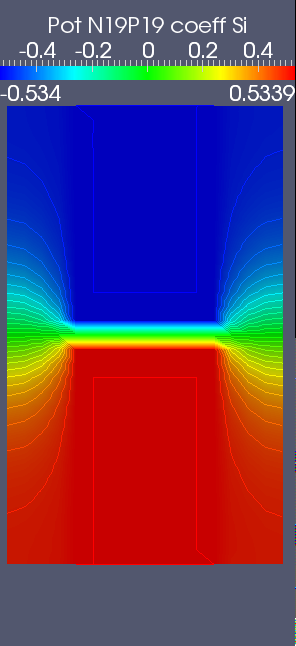
\includegraphics[scale=0.24]{N19P19coeffSiSLICE}}
          \end{figure}
\end{center}
\end{column}

\begin{column}{0.3 \textwidth}
\begin{center}
\begin{figure}[!h]
         \subfigure[Coeff Ox]
          {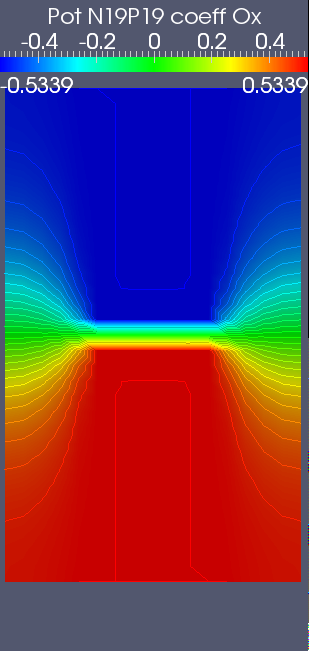
\includegraphics[scale=0.24]{N19P19coeffOxSLICE}}
\end{figure}
\end{center}
\end{column}

\begin{column}{0.3 \textwidth}
\begin{center}
\begin{figure}[!h]
         \subfigure[Sdevice]
          {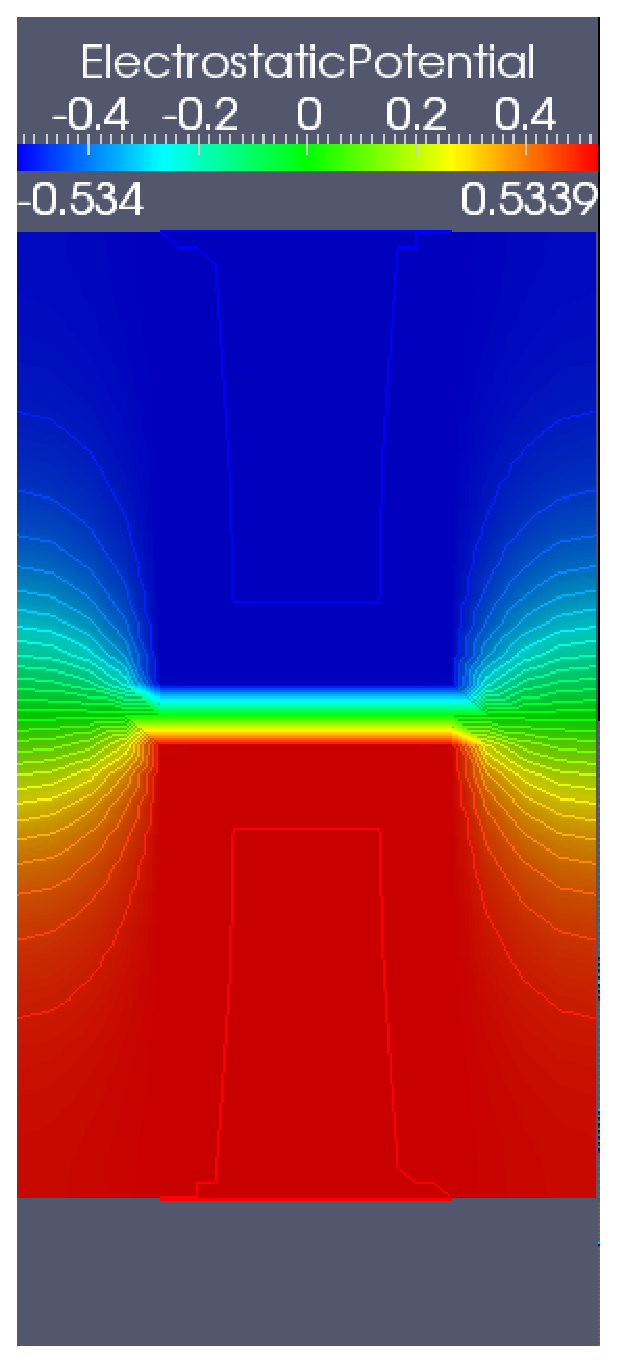
\includegraphics[scale=0.24]{N19P19sdeviceSLICE}}
\end{figure}
\end{center}
\end{column}

\end{columns}

\end{frame}


\begin{frame}
\frametitle{Potenziale tagli N19P19}

\begin{columns}

\begin{column}{0.25 \textwidth}
\begin{center}
\begin{figure}[!h]
         \subfigure[Z=0 Y=0.15]
          {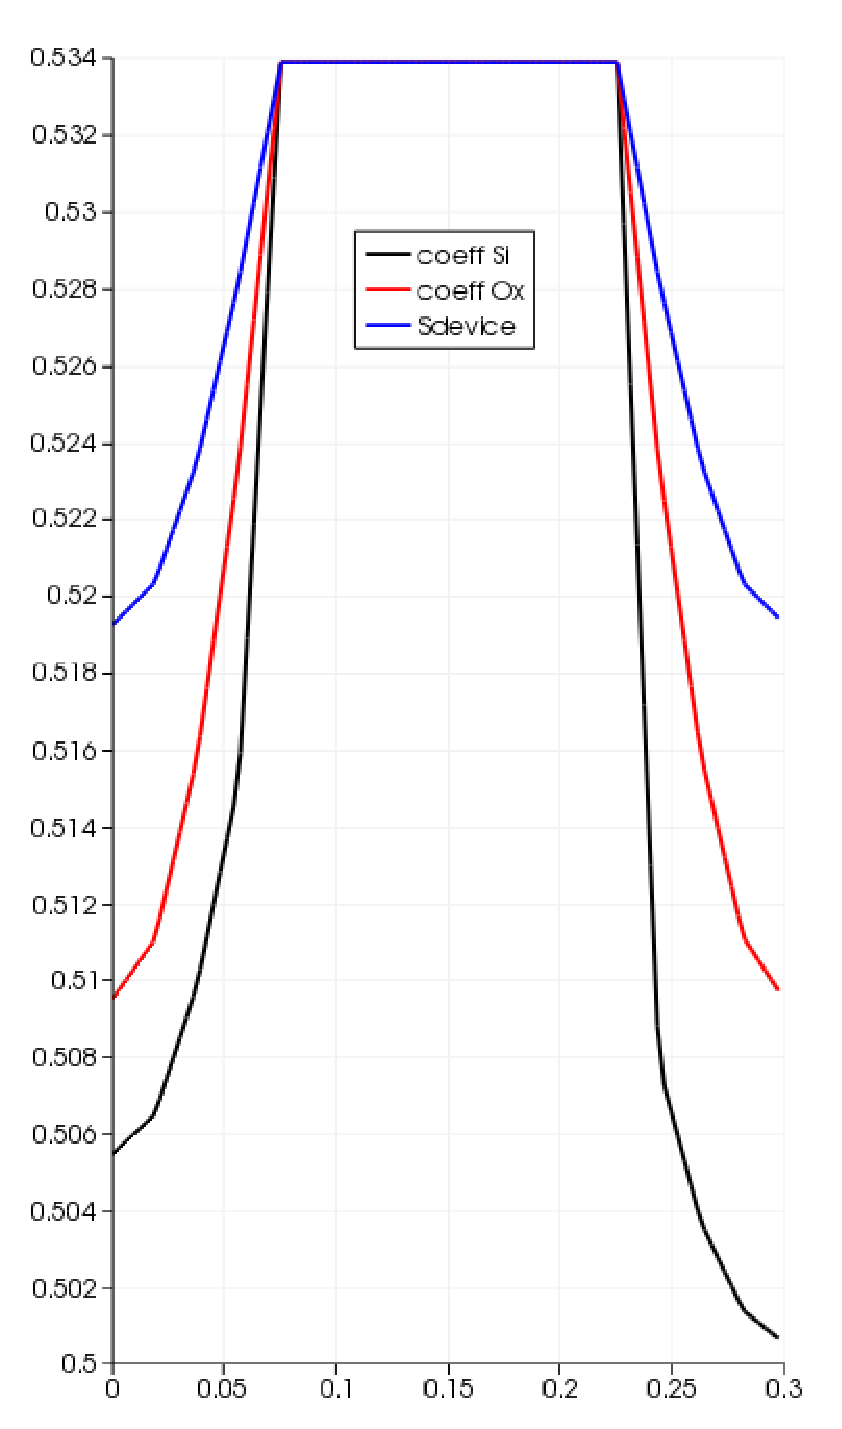
\includegraphics[scale=0.2]{N19P19_Z00Y015}}
          \end{figure}
\end{center}
\end{column}

\begin{column}{0.25 \textwidth}
\begin{center}
\begin{figure}[!h]
         \subfigure[Y=0.15 Z=0.2]
          {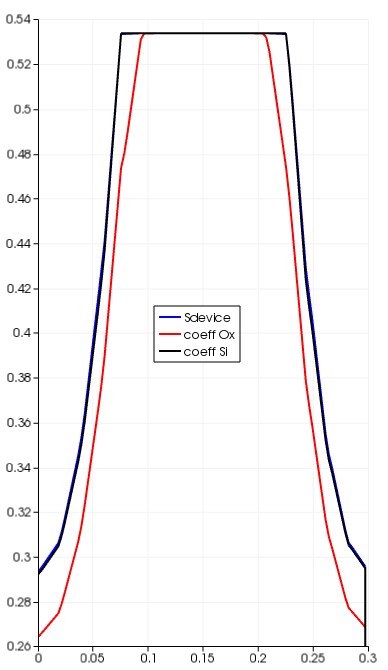
\includegraphics[scale=0.2]{N19P19_Z02}}
\end{figure}
\end{center}
\end{column}

\begin{column}{0.25 \textwidth}
\begin{center}
\begin{figure}[!h]
         \subfigure[X=0.01 Z=0.2]
          {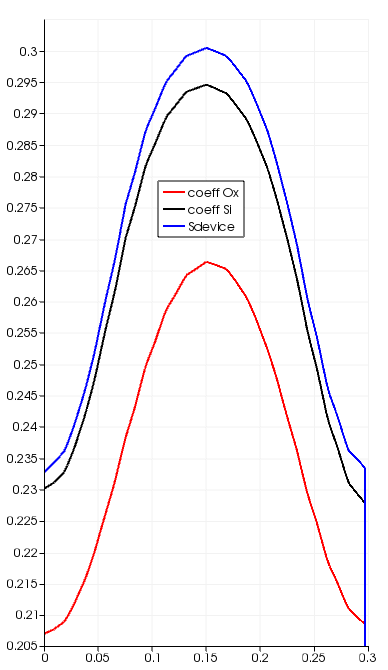
\includegraphics[scale=0.2]{N19P19_Z02X001}}
\end{figure}
\end{center}
\end{column}

\begin{column}{0.25 \textwidth}
\begin{center}
\begin{figure}[!h]
         \subfigure[X=0.01 Z=0.02]
          {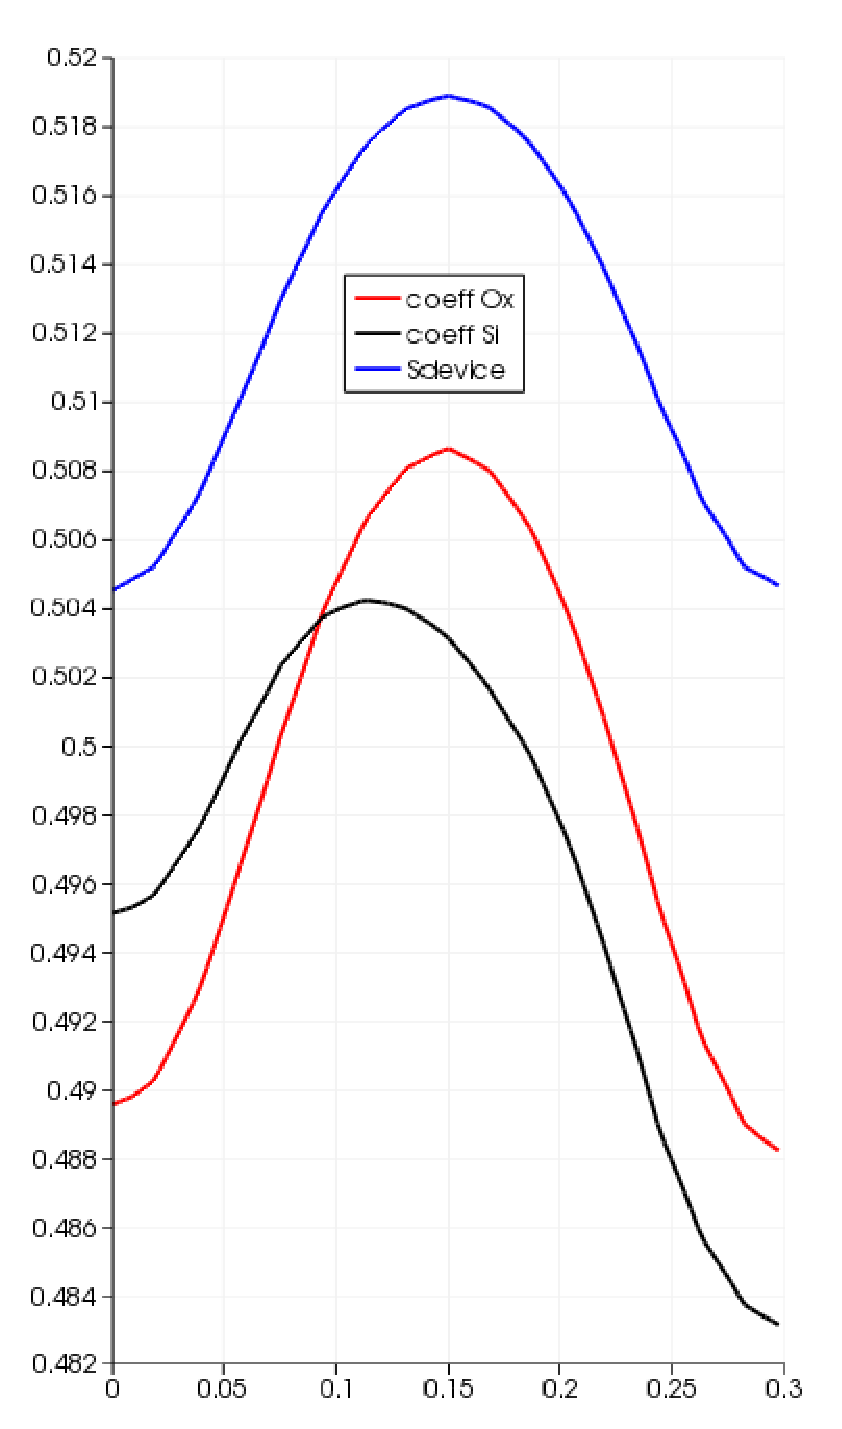
\includegraphics[scale=0.2]{N19P19_Z002Y001}}
\end{figure}
\end{center}
\end{column}

\end{columns}
\end{frame}

%----------------------------------------


\begin{frame}
\frametitle{Potenziale N19P19}
\begin{columns}

\begin{column}{0.3 \textwidth}
\begin{center}
\begin{figure}[!h]
          {\includegraphics[scale=0.25]{PNOX/N19P19/PotentialCoeffSI}}
          \end{figure}
\end{center}
\end{column}

\begin{column}{0.3 \textwidth}
\begin{center}
\begin{figure}[!h]
          {\includegraphics[scale=0.25]{PNOX/N19P19/PotentialCoeffOX}}
\end{figure}
\end{center}
\end{column}

\begin{column}{0.3 \textwidth}
\begin{center}
\begin{figure}[!h]
          {\includegraphics[scale=0.25]{PNOX/N19P19/PotentialSdevice}}
\end{figure}
\end{center}
\end{column}

\end{columns}

\end{frame}

\begin{frame}
\frametitle{Potenziale tagli N19P19}
\begin{columns}

\begin{column}{0.25 \textwidth}
\begin{center}
\begin{figure}[!h]
         \subfigure[X=Y=0.15]
          {\includegraphics[scale=0.2]{PNOX/N19P19/Pot_Y_Z00}}
          \end{figure}
\end{center}
\end{column}

\begin{column}{0.25 \textwidth}
\begin{center}
\begin{figure}[!h]
         \subfigure[X=0.15 Z=0.2]
          {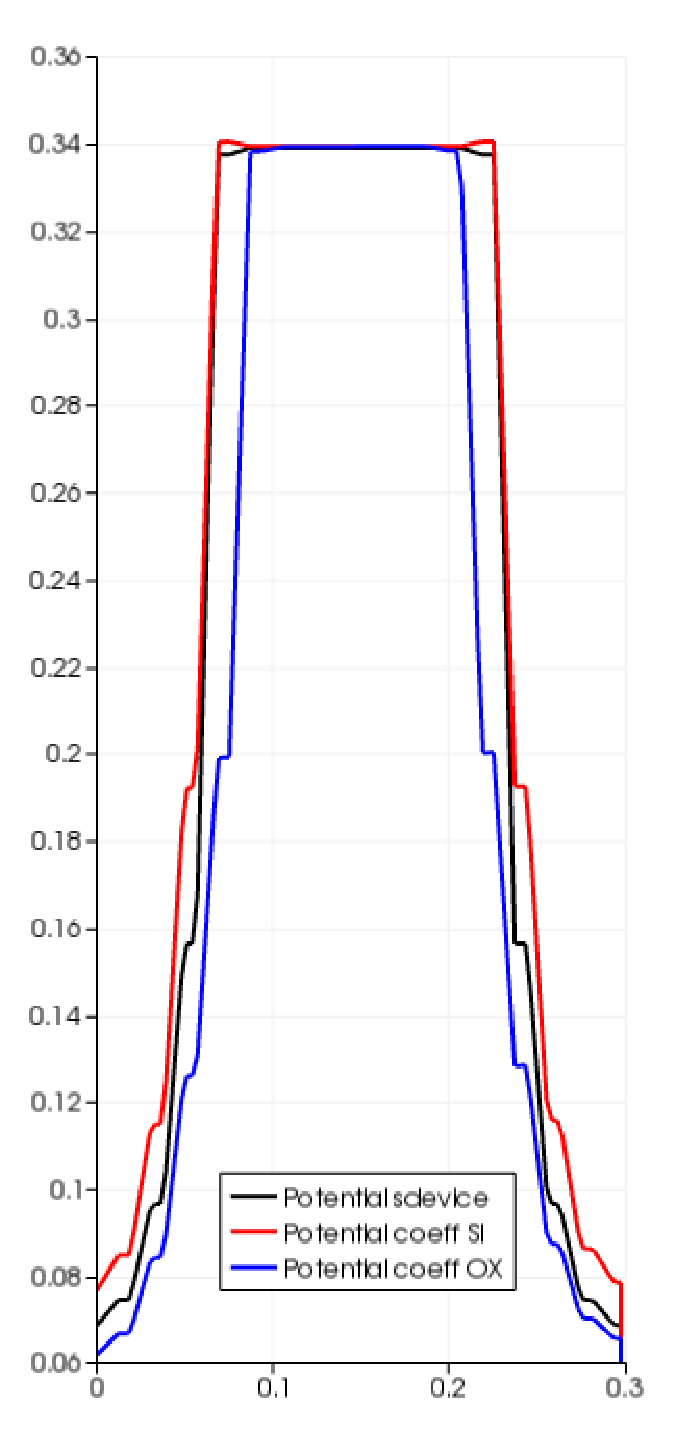
\includegraphics[scale=0.2]{PNOX/N19P19/Pot_Y_Z024}}
\end{figure}
\end{center}
\end{column}

\begin{column}{0.25 \textwidth}
\begin{center}
\begin{figure}[!h]
         \subfigure[X=0.005 Z=0.024]
          {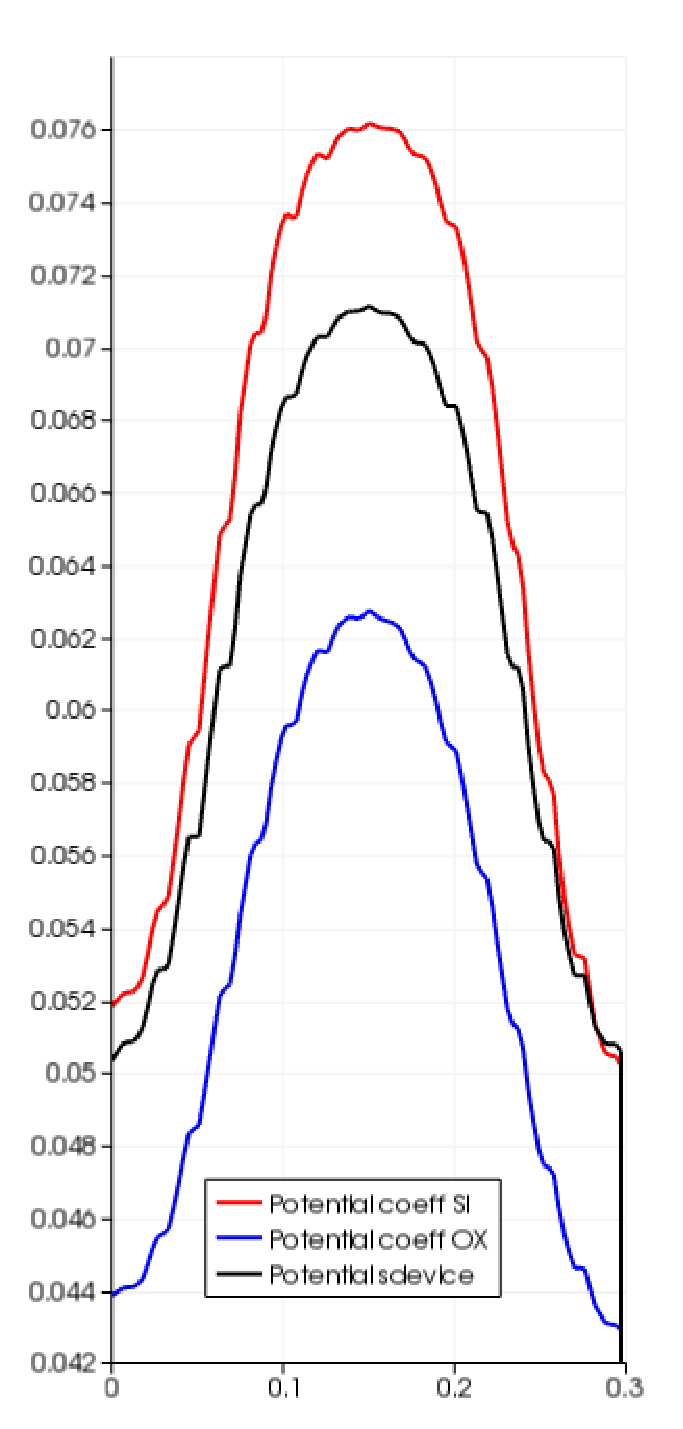
\includegraphics[scale=0.2]{PNOX/N19P19/Pot_Y_Z024X005}}
\end{figure}
\end{center}
\end{column}

\begin{column}{0.25 \textwidth}
\begin{center}
\begin{figure}[!h]
         \subfigure[X=0.0295 Z=0.024]
          {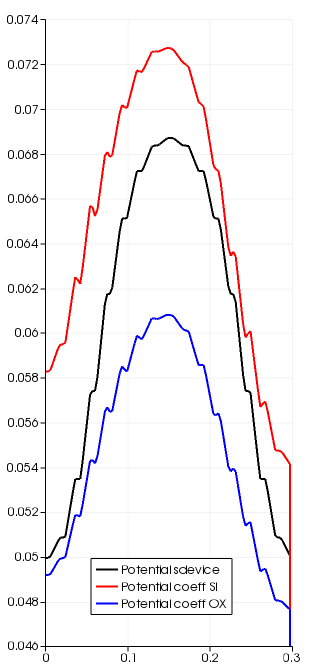
\includegraphics[scale=0.2]{PNOX/N19P19/Pot_Y_Z024X0295}}
\end{figure}
\end{center}
\end{column}

\end{columns}
\end{frame}

